\documentclass[12pt]{article}
\usepackage{amsmath}
\usepackage{enumerate}
\usepackage{mathrsfs} 
\usepackage{amsthm}
\usepackage{amsfonts}
\usepackage{amssymb}
\usepackage{latexsym} 
%\usepackage{epsfig}
%\usepackage{graphicx}
%\usepackage[dvips]{graphicx}
\usepackage{tikz}
\usepackage{tikz-cd}



\usepackage[matrix,tips,graph,curve]{xy}

\newcommand{\mnote}[1]{${}^*$\marginpar{\footnotesize ${}^*$#1}}
\linespread{1.065}

\makeatletter

\setlength\@tempdima  {5.5in}
\addtolength\@tempdima {-\textwidth}
\addtolength\hoffset{-0.5\@tempdima}
\setlength{\textwidth}{5.5in}
\setlength{\textheight}{8.75in}
\addtolength\voffset{-0.625in}

\makeatother

\makeatletter 
\@addtoreset{equation}{section}
\makeatother


\renewcommand{\theequation}{\thesection.\arabic{equation}}

\theoremstyle{plain}
\newtheorem{theorem}[equation]{Theorem}
\newtheorem{corollary}[equation]{Corollary}
\newtheorem{lemma}[equation]{Lemma}
\newtheorem{proposition}[equation]{Proposition}
\theoremstyle{definition}
\newtheorem{definition}[equation]{Definition}
\newtheorem{definitions}[equation]{Definitions}
%\theoremstyle{remark}

\newtheorem{remark}[equation]{Remark}
\newtheorem{remarks}[equation]{Remarks}
\newtheorem{exercise}[equation]{Exercise}
\newtheorem{example}[equation]{Example}
\newtheorem{examples}[equation]{Examples}
\newtheorem{notation}[equation]{Notation}
\newtheorem{question}[equation]{Question}
\newtheorem{assumption}[equation]{Assumption}
\newtheorem*{claim}{Claim}
\newtheorem{answer}[equation]{Answer}
%%%%%% letters %%%%

\newcommand{\fa}{\mathfrak{a}}
\newcommand{\fb}{\mathfrak{b}}
\newcommand{\fm}{\mathfrak{m}}
\newcommand{\fp}{\mathfrak{p}}
\newcommand{\fq}{\mathfrak{q}}

\newcommand{\IA}{\mathbb{A}}
\newcommand{\IN}{\mathbb{N}}
\newcommand{\IP}{\mathbb{P}}
\newcommand{\IZ}{\mathbb{Z}}

\newcommand{\sO}{\mathcal{O}}

\newcommand{\shF}{\mathscr{F}}
\newcommand{\shG}{\mathscr{G}}
%%%%%%% macros %%%%%

%% my definitions %%%

\newcommand{\End}{\mathrm{End}}
\newcommand{\tr}{\mathrm{tr}}
\newcommand{\Hom}{\mathrm{Hom}}
\newcommand{\Aut}{\mathrm{Aut}}
\newcommand{\Trace}{\mathrm{Trace}\,}
\newcommand{\rank}{\mathrm{rank}}
\renewcommand{\deg}{\mathrm{deg}\,}
\newcommand{\Spec}{\rm Spec\,}
\newcommand{\Sym}{\mathrm{Sym \,}}
\newcommand{\Span}{\mathrm{Span \,}}
\renewcommand\dim{{\rm dim\,}}
\renewcommand\det{{\rm det\,}}
\newcommand{\sing}{{\rm sing}}


\newcommand\iso{{\, \cong \,}} 
\newcommand\tensor{{\otimes}}
\newcommand\Tensor{{\bigotimes}} 
\newcommand\union{\bigcup} 
\newcommand\onehalf{\frac{1}{2}}
\newcommand\trivial{{\mathbb I}}
\newcommand\wb{\overline}

%%%%%Delimiters%%%%

\newcommand{\<}{\langle}
\renewcommand{\>}{\rangle}

%\renewcommand{\(}{\left(}
%\renewcommand{\)}{\right)}


%%%% Different kind of derivatives %%%%%

\newcommand{\delbar}{\bar{\partial}}
\newcommand{\pdu}{\frac{\partial}{\partial u}}
%\newcommand{\pd}[1][2]{\frac{\partial #1}{\partial #2}}

%%%%% Arrows %%%%%
\newcommand{\induce}{\rightsquigarrow}
\newcommand{\into}{\hookrightarrow}
\newcommand{\onto}{doubleheadarrow}
\newcommand{\tto}{\longmapsto}
\def\llra{\longleftrightarrow}
\def\wt{\widetilde}
\def\wtilde{\widetilde}
\def\what{\widehat}
\def\bf{\textbf}
\def\it{\textit}
%%%%%%%%%%%%%%%%%%% Ziquan's definitions %%%%%%%%%%%%%%%%%%%%
\newcommand{\Ann}{\mathrm{Ann}}
\newcommand{\height}{\mathrm{height \,}}
\newcommand{\Div}{\mathrm{Div}}
\newcommand{\sE}{\mathcal{E}}
\newcommand{\p}{\partial}
%%%%%%%%%%%%% new definitions for the positive mass paper %%%%%%%%%

\newcommand{\sperp}{{\scriptscriptstyle \perp}}
\newcommand{\st}{\mathrm{s.t.}\,}

%%%%%%%%%%%%%%%%%%%%%%%

%%%%%%%%%%%%%%%%%%%%%%%%%%%%%%%%%%%%%%%%%%%%%



%
\begin{document}
%

\title{Elliptic Surfaces}
\author{Ziquan Yang}


\date{May 14, 2015}

\maketitle
 
%\setcounter{secnumdepth}{1} 

\setcounter{section}{0}

\section{Introduction}
Consider hypersurfaces in $\IP^2 \times \IP^1$ of bidegree $(3, d)$. These hypersurfaces are parametrized by $P = \IP V$, where
$$ V = H^0 ( \IP^2 \times \IP^1, \sO(3, d) ) $$
Let $P^0$ be the subscheme parametrizing those non-singular ones:
$$ P^0 = \{ f \in P : H_f \textit{ is non-singular }\} $$
Let $\pi : \IP^2 \times \IP^1 \to \IP^1$ be projection to the second component. If $H_f$ is non-singular, then fibers of $\pi|_{H_f}$ are cubic curves in $\IP^2$. This makes $H_f$ an elliptic surface. The analogy of being simply ramified for $H_f$ has to do with singular fibers of the map $\pi : H_f \to \IP^1$. Smooth fibers are all isomorphic to the smooth cubic curve. It is customary for some literature to call an irredcucible cubic curve, together with a specified point as the base point, an elliptic curve. There are many types of singular fibers. If the fiber is irreducible, then it is either a nodal curve (e.g. $y^2 = x^2 - x^3$), or a cuspidal curve (e.g. $y^2 = x^3$). If the fiber is not irreducible, then it may be a union of a conic curve and a line, or a union of three lines and there are many different configurations of irreducible components. 
An analogue of a simply ramified curve would be a hypersurface whose singular fibers are all nodal curves. Why is an analogue would be clear in the discussion of Euler characteristics. Hence we are primarily concerned with the following subset of $P^0$: 
$$ D = \{ f \in P^0 : \textit{all singular fibers of $H_f$ are nodal curves} \}$$

For future use we introduce some notation. Let $X$ be a scheme and $f : X \to Y$ be a morphism. For $P \in Y$, we denote the fiber $f^{-1}(P)$ by $X_P$ when $f$ is clear in the context. We denote the singular locus of $X$ by $X_\sing$. If $X \subseteq \IP^n$ and $Q \in \IP^n$, we denote the tangent cone of $X$ at $Q$ by $TC_Q(X)$. If $Q \not\in X$, then $TC_Q(X) = \IP^n$. 

\section{Euler Characteristic}
Just like the genus of a curve tells us the degree of the ramification divisor for a curve of bidegree $(n, d)$ in $\IP^1 \times \IP^1$, the Euler characteristic of a hypersurface in $\IP^2 \times \IP^1$ tells us something about singular fibers. Let $f \in P^0$ and $H_f$ be the corresponding hypersurface. With respect to the map $\pi : H_f \to \IP^1$ we may write $X$ as $X^0 \coprod C$, where $C$ is the finite set of points with singular fibers and $X^0$ is its complement, and $Y$ as $Y^0 \coprod \pi^{-1}(C)$, where $Y^0 = \pi^{-1} X^0$. Let $F$ be the smooth cubic curve in $\IP^2$, we see that $Y^0$ is a $F$-bundle of $X^0$, and their Euler characteristics are related by 
$$ e(Y^0) = e(X^0 ) \cdot e(F) $$ 
Since $e(F) = 0$ we have that $e(Y^0) = 0$. Now since $Y = Y^0 \coprod \pi^{-1}(C)$, we see that $e(Y) = e(Y^0) + e(\pi^{-1}(C)) = e(\pi^{-1}(C))$. Note that $C$ is a finite set of points, and hence $\pi^{-1} (C)$ is a disjoint union of singular cubic curves. 

\begin{figure}[h!]
  \centering
      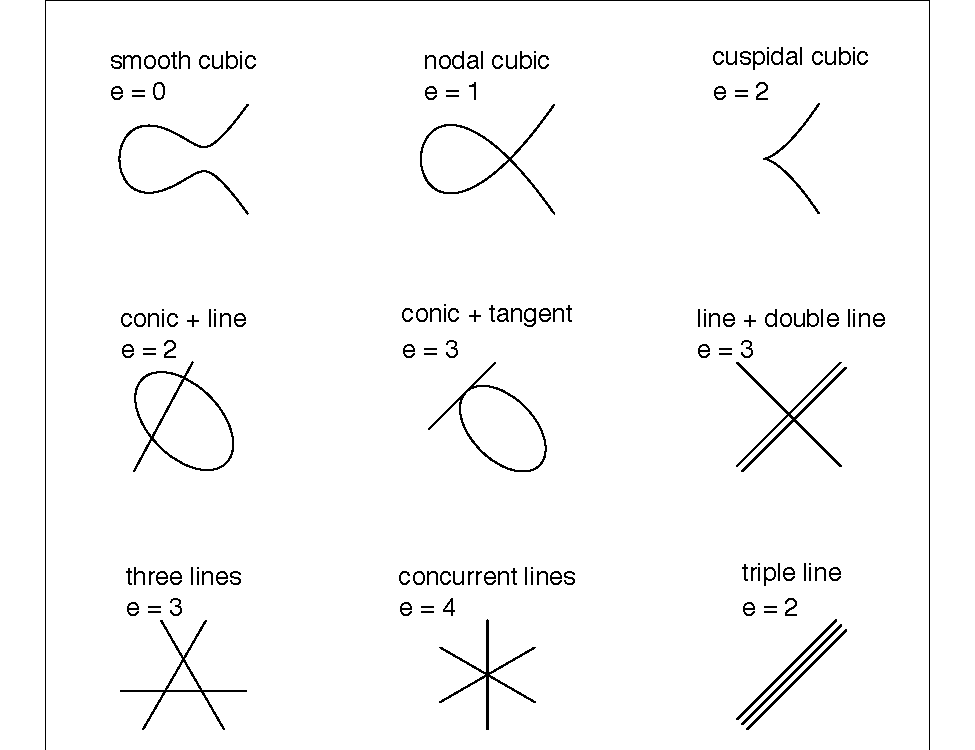
\includegraphics[width=1.0\textwidth]{planecubics}
  \caption{Cubic plane curves and their Euler characteristics \cite{Pic}}
\end{figure}
From the table we see that if $f \in D$, then $e(H_f)$ is exactly the number of points in $\IP^1$ over which the fibers are singular. In this sense, these hypersurfaces are analogues of simply ramified curves in $\IP^1 \times \IP^1$. 

Now we compute $e(H_f)$. In fact we do a more general computation, since it is not harder. Let $H_f \subseteq \IP^2 \times \IP^1$ be a smooth hypersurface of bidegree $(n, d)$. We denote the projections of $\IP^2 \times \IP^1$ onto the first and second components by $\pi_1, \pi_2$ respectively. Let $H_1$ be a hyperplane of $\IP^2$ and $H_2$ be a hyperplane of $\IP^1$. We think of them as generators of the Chow groups of their respective projective schemes. We define 
$$ A = \pi_1^*(H_1), \, E = \pi_2^*(H_2) $$
and $$ h_1 = A \cap H_f, \, h_2 = E \cap H_f $$
We compute the Chern classes of $H_f$ using the standard exact sequence:
$$ 0 \to T_{H_f} \to T_{\IP^2 \times \IP^1|_{H_f}} \to N_{H_f/\IP^2 \times \IP^1} \to 0$$
By Whitney\rq{}s formula, their total Chern classes are related by
$$ c(T_{\IP^2 \times \IP^1|_{H_f}}) = c(T_{H_f}) c(N_{H_f/\IP^2 \times \IP^1}) $$
Now $T_{\IP^2 \times \IP^1|_{H_f}}$ is $T_{\IP^2 \times \IP^1} = \pi_1^* T_{\IP^2} \oplus \pi_2^* T_{\IP^1}$ restricted to $H_f$, so we obtain 
$$ c(T_{\IP^2 \times \IP^1|_{H_f}}) = (1 + 3h_1 + 3h_1^2)(1 + 2h_2) $$
If $\iota : H_f \into \IP^2 \times \IP^1$ is the inclusion, then $$N_{H_f/\IP^2 \times \IP^1} = \iota^* \sO_{\IP^2 \times \IP^1}(nA  + dE) = (1 + nh_1 + dh_2)$$
Therefore 
\begin{align*}
c(T_{H_f}) &= c(T_{\IP^2 \times \IP^1|_{H_f}})c(N_{H_f/\IP^2 \times \IP^1})^{-1}\\
&= (1 + 3h_1 + 3h_1^2)(1 + 2h_2)(1 + nh_1 + dh_2)^{-1}\\
&= (1 + 3h_1 + 3h_1^2)(1 + 2h_2)(1 - (nh_1 + dh_2) + (nh_1 + dh_2)^2 - \cdots)
\end{align*}
In particular we obtain 
$$ c_2(T_{H_f}) = (n^2 - 3n + 3)h_1^2 + (6 + 2nd - 2n - 3d)h_1 h_2 $$
which is the top Chern class. Now we compute 
\begin{align*}
\deg h_1^2 &= A \cdot A \cdot (nA + dE) = d \\
\deg h_1 h_2 &= A \cdot E \cdot (nA + dE) = n 
\end{align*}
Finally we obtain 
$$ e(H_f) = \deg c_2(T_{H_f}) = 6n + 3d + 3n^2 d - 6 dn - 2n^2 $$
In particular, for future use we want to fix $n = 3$, so $e(H_f)$ depends only on $d$. In this case $e(H_f) = 12 d$.  

\section{An Analogue of Bertini\rq{}s Theorem}
Let $k$ be algebraically closed. We show an analogue of Bertini's theorem: 
\begin{theorem}
$D$ is a constructible subset of $\IP V$, and $D \neq \IP V$. 
\end{theorem}
Let $X = \IP^2 \times \IP^1$. In this section by ``fiber" the underlying morphism is always the projection $\pi : X \to \IP^1$, or its restrictions. We define 
$$ R = \{ f \in \IP V : \exists P \in \IP^1, \st (H_f)_P \textit{ is reducible} \} $$
and 
$$ C = \{ f \in \IP V : \exists P \in \IP^1, Q \in X_P, \st Q \in ((H_f)_P)_\sing \textit{ and } TC_Q((H_f)_P) \textit{ is a line}\}$$
Note that $C - R$ parametrizes those hypersurfaces $H_f$ that have some singular fiber isomorphic to a cuspidal curve. Therefore if $D' = \IP V - R \cup C$, then $D = D' \cap P^0$. It suffices to show that $R, C$ are both constructible, and $\dim R, \dim C < \dim \IP V$. 

\begin{lemma}
$R$ is constructible and $\dim R < \dim \IP V$. 
\end{lemma}
\begin{proof}
By Bezout's theorem, if a curve of degree three intersects a line with multiplicity $\ge 4$, then it has to contain the line as an irreducible component. Conversely, if a degree 3 curve is reducible, then it contains a line as an irreducible component. Moreover, a reducible degree 3 curve is singular and the singularity must lie on the line. In order to better motivate the later arguments, we first do some examples. Let $(x_0 : x_1 : x_2)$ be the homogeneous coordinate on $\IP^2$. Then for for any pair $(L, P)$, where $L$ is a line in $\IP^2$ and $P$ is a point, there is at least one of the charts $\IA_i = \{ x_i  \neq 0 \}$ covers all but at most one point of the line $L$ and contains $P$. Consider the chart $\IA_2 \times \IA \subseteq X$. Let $t$ be the coordinate of $\IA$, then $f \in \IP V$ can be written in the form,
$$ f = \sum_{0 \le i + j \le 3} f_{ij}(t) x_0^i x_1^j, \text{ where } f_{ij} = \sum_{0 \le k \le d} a_{ijk} t^k $$
If $H_f \subseteq X$ is smooth, then for any $P \in \IA$, $f_P = \sum f_{ij}(P) x_0^i x_1^j$ is the dehomogenization at $x_2 \neq 0$ of some degree $3$ curve. $f_P$ itself, however, may not be of degree $3$. In fact, it is possible that a homogeneous polynomial of degree $3$ in $H^0(\IP^2, \sO_{\IP^2}(3))$ does not give a degree $3$ polynomial under any of the dehomogenization at $\IA_i$'s. Therefore we are not guaranteed to see any of the pictures in the previous page on any of the affine charts. However, this does not matter. We only need to see a line through a singular point in one of the affine charts for our purposes. 

Suppose for some $f$ and $P$, we have $f_P = y(y - x^2)$. We can detect that it contains the x-axis as an irreducible component by looking at its derivatives:
$$ f(0, 0) = 0; \frac{\p }{\p x} f(0, 0) = 0 ; \frac{\p^2 }{\p x^2} f(0, 0) = 0; \frac{\p^3 }{\p x^3} f(0, 0) = 0 $$
since the above equations implies at the curve $C_{f_P} : \{ f_P = 0 \}$ intersects the line $y = 0$ at $(0, 0)$ with multiplicity $\ge 4$. 

Now suppose some $f_P = (y - x)(y - 2x) = y^2 - 3xy + 2x^2$ Clearly the curve is singular at $(0, 0)$. Suppose it has contains a line of the form $y + ax = 0$. We may perform a change of variables:
\begin{align*}
u &= y + ax \\
v &= y + (a - 1) x
\end{align*}
Coversely,
\begin{align*}
x &= u - v \\
y &= (1 - a)u + av
\end{align*}
To require that $C_{f_P}$ intersects the line $y + ax = 0$ with multiplicity $\ge 4$ is to impose conditions:
\begin{align*}
f (u - v, (1 - a)u + av)|_{u = 0, v= 0}&= 0 \\
\frac{\p }{\p u}\big|_{u=0, v=0}  f (u - v, (1 - a)u + av)&= 0 \\
\frac{\p^2 }{\p u^2}\big|_{u=0, v=0}  f (u - v, (1 - a)u + av)&= 0 \\
\frac{\p^3 }{\p u^3}\big|_{u=0, v=0}  f (u - v, (1 - a)u + av)&= 0
\end{align*}
In general, in circumstances like this, the first two equations are always satisfied, since $C_{f_P}$ is assumed to have a singular point at $Q$ (in this case $(0, 0)$) from the first place. In this particular example, the last equation is 



Therefore, in order to apply the classical Bertini argument, we consider a subscheme of 
$$ \IP^1 \times (\IA^2 \times \IA^1 ) \times \IP V $$
We use the middle term $\IA^2 \times \IA^1$ in intended to be an open affine chart on $X$, and the first $\IP^1$ component to parametrizes directions through a give points in $X$. Let the coordinates of the above scheme by given by 
$$( (a_0 : a_1) , (x_0, x_1), t, (a_{ijk})_{0 \le i + j \le 3, 0 \le k \le d} ) $$ 

Roughly speacking, we want to describe a subscheme 
$$ G = \{ (\lambda, Q, P, f) \in \IP^1 \times (\IA^2 \times \IA^1 ) \times \IP V : Q \in ((H_f)_P)_\sing \textit{ and } ((H_f)_P \cdot l_{Q, \lambda})_Q \ge 4\} $$
$l_{Q, \lambda}$ means the line through $Q$ with direction normal to $\lambda$, i.e. if $Q = (q_0, q_1) \in \IA^2$, $\lambda = (a_0 : a_1)$, then $l_{Q, \lambda}$ is the line $a_0 x_0 + a_1 x_1 - (a_0 q_0 + a_1 q_1) = 0$
\end{proof}


%% \section{Discussion}
%% \subsection{Alternative dimension counting method}
The above proof once again shows the robustness of Poonen's decoupling idea. We may modify it to decouple higher power derivatives, mixed partials, almost whatever we need. However, the method also heavily depends on the linearity of conditions. For example, we cannot directly decouple the condition 
$$ (f_{xy})^2 = f_{xx} f_{yy} $$
in ruling off double lines. Instead, we need to make it linear by introducing an auxilliary variable. In fact, our proof in section 3 is deliberately set up as a preparation for the sieve method. If all that we want to do is to show the result itself, we could have done the dimension counting in an eaiser way, without resorting to Taylor expansion and tangent cones. Here we present the proof:

5 However, the drawback of the proof is that it does not directly translates to a sieve method for schemes over finite fields. 
%% \subsection{Change of variable}
%% My original plan to attack the problem was not to studying how the homogeneous components (after Taylor expansion) factor, but instead to actively search for a line such that the curve intersects with multiplicity $\ge 4$. For example, to test whether the line $y = 0$, i.e. $x$-axis is an irreducible component of a degree $3$ planar curve through the origin $(0, 0)$ described by $f \in \IF_q[x, y]$, $\deg f = 3$, then it suffices to check that 
%% $$ f(0, 0) = \frac{\p f}{\p y} (0, 0) = \frac{\p^2 f}{\p y^2} (0, 0) = \frac{\p^3 f}{\p y^3} (0, 0) = 0$$
%% Bezout theorem will force $y = 0$ to be an irreducible component of $f= 0$. However, we can also see this without resorting to Bezout's theorem. Some elementary computation will show that that if we write $f = \sum_{0 \le i + j \le 3} a_{ij}x^i y^j$ then the above equations will force that $a_{00} = a_{01} = a_{02} = a_{03} = 0$ and hence $x \mid f$. 
%% Abstractly the intersection multiplicity of two curves $C = \{f = 0\}, D = \{g = 0\}$ at $(x_0, y_0)$ can be computed by 
%% $$ (C \cdot D)_{(x_0, y_0)} = \dim_{\IF_q} \IF_q[x, y]_{(x_0,y_0)}/(f, g) $$
%% Therefore it is clear that intersection multiplicity is invariant under invertible change of variables (i.e. those that induce isomorphisms on $\IF_q[x, y]$), and in particular under linear change of variables with a nonzero determinant.  
%% \subsection{Order of singularity}

\begin{thebibliography}{9}
\bibitem{Pic}
B. Poonen, An explicit algebraic family of genus-one curves violating the Hasse principle, available at \textit{http://www-math.mit.edu/~poonen/}


\end{thebibliography}
                                                                                                                                                                                                                                                                                                                                                                                                                                                                                                                                                                                                                                                                                                                                                                                                                                                                                                                                                                                                                                                                                                                                                                                                                                                                                                                                                                                                                                                                                                                                                                                                                                                                                                                                                                                                                                                                                                                                                                                                                                                                                                                                                                                                                                                                                                                                                                                                                                                                                                                                                                                                                                                                                                                                                                                                                                                                                                                                                                                                                                                                                                                                                                                                                                                                                                                                                                                                                                                                                                                                                                                                                                                                                                                                                                                                                                                                                                                                                                                                                                                                                                                                                                                                                                                                                                                                                                                                                                                                                                                                                                                                                                                                                                                                                                                                                                                                                                                                                                                                                                                                                                                                                                                                                                                                                                                                                                                                                                                                                                                                                                                                                                                                                                                                                                                                                                                                                                                                                                                                                                                                                                                                                                                                                                                                                                                                                                                                                                                                                                                                                                                                                                                                                                                                                                                                                                                                                                                                                                                                                                                                                                                           


\end{document}